\newpage
\section{Exercises}
\newcounter{qcounter}
\begin{list}{
\textbf{Question \arabic{qcounter}:}~}{\usecounter{qcounter}}

\iffalse
\item \noindent The perceptron model was one of the first neural network algorithms. One of the limitations that made its application difficult was the restriction of not operating on non-linearly separable problems. This limitation was mainly known when used to simulate logical gates. Computationally assemble the perceptron model to simulate the three types of logic gates (AND, OR, XOR) and comment on the results considering the limitations of the perceptron.


\item \noindent  Based on the MLP network architecture in the figure, construct the MLP network computationally.
\begin{figure}
    \centering
    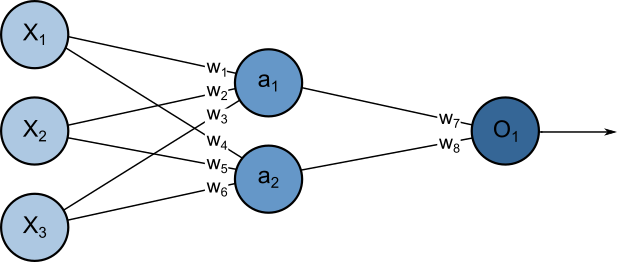
\includegraphics[scale=0.65]{images/backpropagation_ex.png}
    \caption{Simple neural network}
    \label{fig:exercise7}
\end{figure}

\item \noindent The Figure \ref{fig:exercise7} shows a simplified neural network architecture. Do the first backpropagation pass, whereas in the first forward pass, the following operations were made:

$$X \texttt{=}
\left[\begin{smallmatrix}
4 & 3 & 5
\end{smallmatrix}\right]
, 
\text{Desired output}
\texttt{=}
\left[\begin{smallmatrix}
1
\end{smallmatrix}\right]
, 
\left[\begin{smallmatrix}
\text{w}_1 & \text{w}_4\\
\text{w}_2 & \text{w}_5 \\
\text{w}_3 & \text{w}_6
\end{smallmatrix}\right]
\texttt{=}
\left[\begin{smallmatrix}
0.12 & 0.33\\
0.5 & 0.7 \\
0.15 & 0.45
\end{smallmatrix}\right]
\text{and}
\left[\begin{smallmatrix}
\text{w}_7 \\
\text{w}_8
\end{smallmatrix}\right]
\texttt{=}
\left[\begin{smallmatrix}
0.13 \\
0.6
\end{smallmatrix}\right]
$$

$$\left[\begin{smallmatrix}
4 & 3 & 5
\end{smallmatrix}\right]
\cdot 
\left[\begin{smallmatrix}
0.12 & 0.33\\
0.5 & 0.7 \\
0.15 & 0.45
\end{smallmatrix}\right]
=
\left[\begin{smallmatrix}
2.73 & 5.67 
\end{smallmatrix}\right]
\rightarrow
\text{sigmoid}(\left[\begin{smallmatrix}
2.73 & 5.67 
\end{smallmatrix}\right])
=
\text{a}
=
\left[\begin{smallmatrix}
0.94 & 0.99 
\end{smallmatrix}\right]
$$

$$\left[\begin{smallmatrix}
0.94 & 0.99 
\end{smallmatrix}\right]
\cdot 
\left[\begin{smallmatrix}
0.13\\
0.6 
\end{smallmatrix}\right]
=
\left[\begin{smallmatrix}
0.71
\end{smallmatrix}\right]
\rightarrow
\text{sigmoid}(\left[\begin{smallmatrix}
0.71
\end{smallmatrix}\right])
=
\text{O}_1
= 
\left[\begin{smallmatrix}
0.67
\end{smallmatrix}\right]
$$

$$
\text{Error}
=
\frac{1}{2}(0.67-1.0)^2=0.05445
$$


\item The MNIST dataset contains images of numbers from 0 to 9, with each of these images being $28$x$28$ in size. Implement a neural network to sort the digits, considering that the input will have a dimension of $28$x$28=784$, use $30$ nodes in the hidden layer and finally $10$ positions in the output. Once implemented, perform tests varying the number of epochs and the amount of data to evaluate the accuracy behavior using graphics.


\item There are different error functions that can be used during the training of a neural network, as an example we have the cross entropy, the mean square error, among others. Considering the network implemented in the previous exercise, choose another error function to change the algorithm and then compare the results of the two models.
\fi

\item \noindent Considering the focus on convolutional neural networks, we can highlight convolution as a basic operator. For a basic understanding of the application and effect of convolution, manually convolute the $\left[\begin{smallmatrix}
0 & 2 & 3\\
0 & 1 & 0\\
3 & 0 & 2
\end{smallmatrix}\right]$ onto the $\left[\begin{smallmatrix}
1 & 2 & 0\\
3 & 0 & 0\\
4 & 1 & 0
\end{smallmatrix}\right]$ and compare with the computationally calculated result. 


\item \noindent The combination of convolutions allows networks to learn at different levels of information about the object of study. In the context of applications with images, each convolution layer can identify a level of detail, for example, in the initial layers there are more general elements of the images, such as lines, edges and corners. Some filters, or convolutions, that have the edge detection property are Sobel and Prewitt. Apply each filter to an image and compare the results.


\begin{itemize}
\item Prewitt Operators. By applying each operator on the image and performing the sum of the modulus of each result, it is possible to determine the edges in the image.

$G_x= \left[\begin{smallmatrix}
-1 & 0 & 1\\
-1 & 0 & 1\\
-1 & 0 & 1
\end{smallmatrix}\right]$

$G_y = \left[\begin{smallmatrix}
-1 & -1 & -1\\
 0 &  0 &  0\\
 1 &  1 &  1
\end{smallmatrix}\right]$

\item Sobel Operators. By applying each operator on the image and performing the sum of the modulus of each result, it is possible to determine the edges in the image.

$G_x= \left[\begin{smallmatrix}
-1 & 0 & 1\\
-2 & 0 & 2\\
-1 & 0 & 1
\end{smallmatrix}\right]$

$G_y = \left[\begin{smallmatrix}
-1 & -2 & -1\\
 0 &  0 &  0\\
 1 &  2 &  1
\end{smallmatrix}\right]$

\end{itemize}

\item \noindent One of the techniques used in image applications using convolutional neural networks is to reduce the size of inputs across layers, which can reduce computational costs. To perform this reduction we can use strides in the application of convolution. Perform the convolution between kernel $\left[\begin{smallmatrix}
0 & 2 & 3 \\
0 & 1 & 0 \\
3 & 0 & 2 
\end{smallmatrix}\right]$ and matrix  $\left[\begin{smallmatrix}
1 & 2 & 0 & 3 & 0\\
3 & 0 & 0 & 1 & 0\\
4 & 1 & 0 & 2 & 1
\end{smallmatrix}\right]$, first using stride 1 and then with stride 2 to assess the effect of this technique. 


\item \noindent During image processing in convolutional neural networks, there are steps in which the inputs and outputs of the convolution layers need to keep the same size, and one way to have this control is to use padding in the application of the convolution. With the same kernel and matrix as in the previous exercise, determine a padding to ensure that the result remains the same size as the original matrix, and then apply the convolution using this padding.


\item \noindent The LeNeT network is one of the simplest convolutional networks, being possible to implement without the use of frameworks and still obtain good results in a short period of testing time. Using the MNIST dataset build a LeNet network for digit classification, with and without framework. Evaluate the implementation complexity in the two cases and the results considering the same input and training parameters.


\item The construction of a Convolutional Neural Network for classification of cats and dogs images is a very common exercise, usually performed to demonstrate the most important ideas in the functioning of CNNs. That said, use some dataset that contains images of dogs and cats (like the one available in the TensorFlow library\footnote{\url{https://www.tensorflow.org/datasets/catalog/cats_vs_dogs}}) and use it to compare the performance of the AlexNet, VGG and GoogleLeNet networks (remembering that these models are already available, fully pre-trained, in libraries such as Keras\footnote{\url{https://keras.io/api/applications/}} and Pytorch\footnote{\url{https://pytorch.org/vision/stable/models.html}}).


\item As explained in the Transfer Learning section \ref{transferlearning}, Convolutional Neural Networks with large and complex architectures can take a long time and consume large amounts of processing and memory in their training. Using pre-trained networks can help us, as we can use them directly or train them from that point on. Like in the previous exercise, use pre-trained models from some library, but this time using a dataset with a larger number of classes (for example, the cifar100 dataset\footnote{\url{https://www.tensorflow.org/datasets/catalog/cifar100}} that contains 100 classes). Also check the difference in performance of each model, taking into account its complexity and the number of classes.
\end{list}